\documentclass[a4paper,11pt]{article} % Formato do papel, tipo de documento e tamanho da fonte.
\usepackage[utf8]{inputenc}
\usepackage[brazil]{babel} % Hifenização em português
\usepackage[T1]{fontenc} % Caracteres com acentos são considerados como um bloco
\usepackage{ae} % Arruma a fonte quando usa o pacote acima
\usepackage{amssymb} % Caracteres matemáticos especiais
\usepackage[pdftex]{graphicx} % Para inserir figuras    
\usepackage{indentfirst}
\usepackage{float}

\setlength{\parindent}{1cm}
%\renewcommand{\theenumi}{\Alph{enumi}}

\title{
	\vspace{0 mm}
	\huge{\textbf{MAC0438 - Programação Concorrente}} \\
	\vspace{3 mm}
	\huge{EP3 - Jantar dos 'selvagens'}
	\vspace{0 mm}
}

\author	{
	\Large{{ Antônio Martins Miranda - Igor Canko Minotto}}	\\
}
\date{\Large{{ 17 de junho de 2014}}}


\usepackage{graphicx}
\begin{document}

\maketitle
\thispagestyle{empty}
\pagebreak 
\pagenumbering{arabic}
\tableofcontents
\thispagestyle{empty}
\pagebreak
\setcounter{section}{-1}
\setcounter{page}{1}

\section{Introdução}
  Para simular o problema do jantar dos selvagens, utilizamos a linguagem C que, através da biblioteca \textit{pthread}
  possui implementações das funções \textit{wait, signal e signal\_all}. O monitor foi implementado como um módulo 
  (monitor.c). A fila de prioridade foi implementada externamente à biblioteca, por nós.
  
\section{Ambiente}
  Para rodar os testes que geraram os resultados apresentados neste relatório, usamos o seguinte sistema :
\begin{itemize}
\item SO: Ubuntu Linux 12.04 (32-bit)
\item RAM: 6GB
\item Processador: i5 2.50 GHz x 4 cores
\item Compilador C: gcc 4.6.3
\end{itemize}

\section{Método}
  Demos um valor de 1000 repetições para o programa, repetindo a execução 10 vezes para cada caso, paras as opções U e P.

\section{Valores}
  Para os casos 1 e 2, estes foram os valores usados:\linebreak\linebreak
  \centerline{\begin{tabular}{ l }
  2 \\
  1 2 \\
  2 \\
  2 \\
  \end{tabular}}\linebreak\linebreak
  \indent Já para os casos 3 e 4, os valores foram os seguintes:\linebreak\linebreak
  \centerline{\begin{tabular}{ l }
  20 \\
  1 2 3 4 5 6 7 8 9 10 11 12 13 14 15 16 17 18 19 20 \\
  6 \\
  10 \\
  \end{tabular}}
  
\pagebreak
\section{Análise dos Resultados}
  
    No caso 1, o gráfico 1 mantém uma linearidade esperada e as retas para dois cozinheiros se aproximam bastante.
  Além disso, no gráfico 2, as duas barras se aproximam bastante, o que é esperado do caso com pesos uniformes.
  
  \centerline{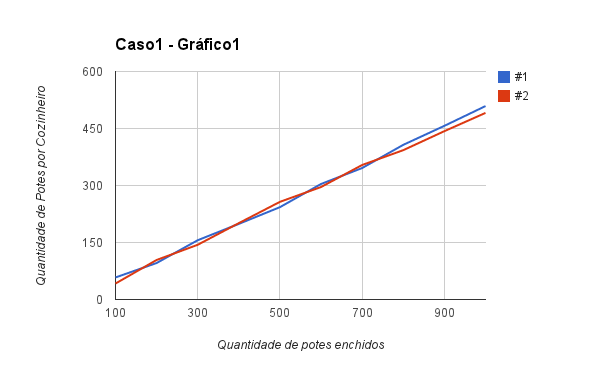
\includegraphics[width=\linewidth]{charts/1-1.png}}
  \centerline{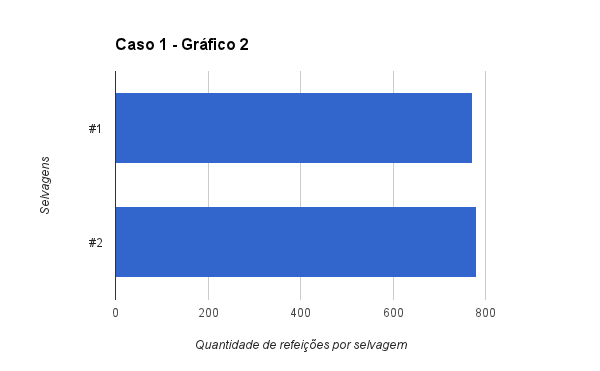
\includegraphics[width=\linewidth]{charts/1-2.png}}
  \pagebreak
  No caso 2, ainda existe uma justiça entre os cozinheiros. Quanto aos selvagens, percebemos que existe uma predileção
  do segundo em relação ao primeiro, mas a proporcionalidade dos pesos não é respeitada. Isso se deve a falhas em nossa
  implementação, as quais não foram indentificadas a tempo da entrega.
  
  \centerline{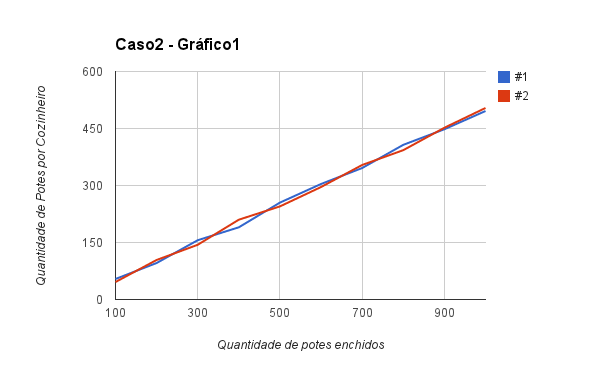
\includegraphics[width=\linewidth]{charts/2-1.png}}
  \centerline{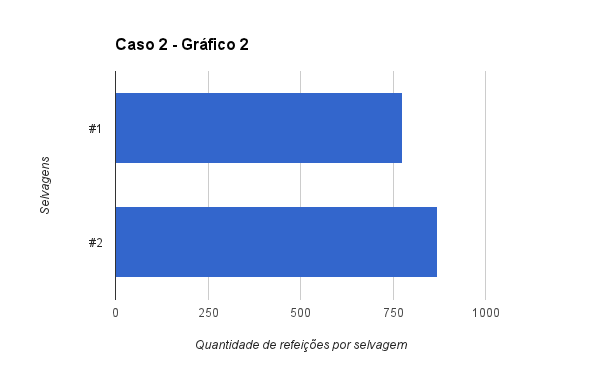
\includegraphics[width=\linewidth]{charts/2-2.png}}
  \pagebreak
  No caso 3, o comportamento é similar ao caso 1, em ambos os gráficos, apenas com maior flutuação nos dados.
  Isto poderia ser amaneziado analisando uma maior amostra de dados.
  
  \centerline{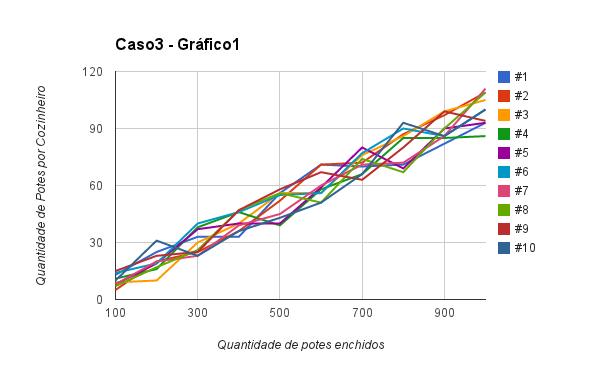
\includegraphics[width=\linewidth]{charts/3-1.png}}
  \centerline{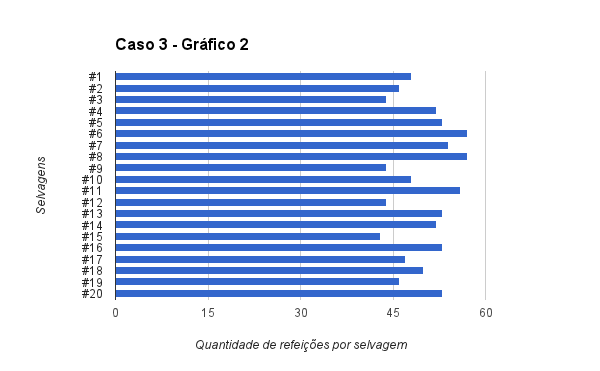
\includegraphics[width=\linewidth]{charts/3-2.png}}
  \pagebreak
  No caso 4, a justiça entre os cozinheiros se mantém, novamente. Mas aqui, diferente do caso 2, podemos ver mais
  claramente a proporção entre o número de refeições de um selvagem e seu peso.
  
  \centerline{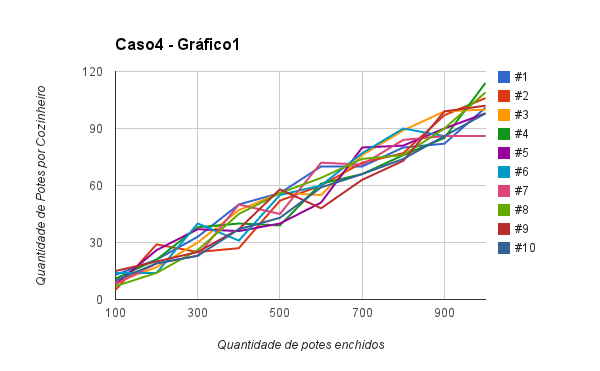
\includegraphics[width=\linewidth]{charts/4-1.png}}
  \centerline{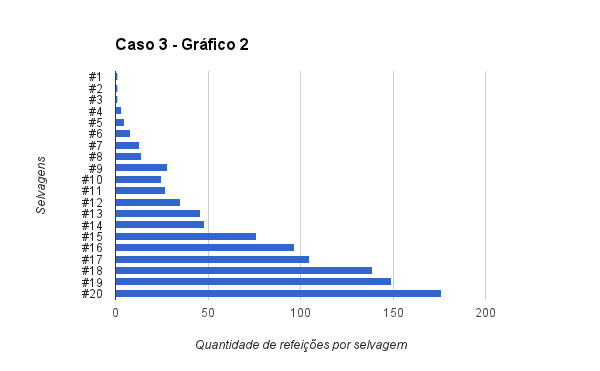
\includegraphics[width=\linewidth]{charts/4-2.png}}
  
\end{document}

